% HMC Math dept HW template example
% v0.04 by Eric J. Malm, 10 Mar 2005
\documentclass[12pt,letterpaper,boxed,cm]{hmcpset}

% set 1-inch margins in the document
\usepackage[margin=1in]{geometry}
\usepackage{mathtools}
\usepackage{mathrsfs}
% include this if you want to import graphics files with /includegraphics
\usepackage{graphicx}
\usepackage{cases}
\usepackage{hyperref}
\usepackage{siunitx}
\usepackage{tikz}
\usepackage{cases}
\usetikzlibrary{arrows}

% info for header block in upper right hand corner
\name{Name: ~~~~~~~~~~~~~~~~~~~~~~~}
\class{Physics 51}
\assignment{Homework \#8}
\duedate{September 26, 2016}

\newcommand{\ev}[2]{\Big|_{#1}^{#2}}
\newcommand{\evv}[2]{\Big|_{#1}^{#2}}
\newcommand{\set}[1]{\left\{#1\right\}}
\newcommand{\s}[1]{\sqrt{#1}}
\newcommand{\f}[2]{\frac{#1}{#2}}
\newcommand{\p}[2]{\frac{\partial #1}{\partial #2}}
\providecommand{\t}[1]{\text{#1}}
\providecommand{\span}[1]{\text{span}\left(#1\right)}
\providecommand{\set}[1]{\left\{#1\right\}}
\providecommand{\l}[0]{\left}
\providecommand{\r}[0]{\right}
\newcommand{\m}[1]{\begin{matrix}#1\end{matrix}}
\newcommand{\bm}[1]{\begin{bmatrix}#1\end{bmatrix}}
\renewcommand{\bf}[1]{\mathbf{#1}}
\newcommand{\pn}[1]{\left( #1 \right)}
\newcommand{\abs}[1]{\left| #1 \right|}
\newcommand{\bk}[1]{\left[ #1 \right]}
\newcommand{\cis}[1]{\pn{\cos\pn{#1} + i\sin\pn{#1}}}
\newcommand{\cisi}[1]{\pn{\cos\pn{#1} - i\sin\pn{#1}}}
\renewcommand{\Im}[1]{\text{Im}\pn{#1}}
\renewcommand{\Re}[1]{\text{Re}\pn{#1}}
\renewcommand{\k}[0]{\f{1}{4\pi\epsilon_0}}
\renewcommand{\part}[1]{\vspace{1em}\noindent(#1)}

\makeatletter
\renewcommand*\env@matrix[1][*\c@MaxMatrixCols c]{%
  \hskip -\arraycolsep
  \let\@ifnextchar\new@ifnextchar
  \array{#1}}
\makeatother
\begin{document}
\problemlist{SUP11, SUP12, SUP13, SUP27*}

\begin{problem}[SUP11]
 A primitive model of the hydrogen atom consists of a point nucleus ($+e$) surrounded by a uniformly charged spherical cloud ($-e$) of radius $a$. Based on this model, let's calculate the atomic polarizability of hydrogen. Recall that the atomic polarizability, $\alpha$, is defined from $\mathbf{p} = \alpha\mathbf{E}_{\text{ext}}$ where $\mathbf{p}$ is the dipole moment of the atom.
\begin{enumerate}
	\item[(i)] Assume that the applied electric field displaces the center of the electron cloud relative to the nucleus by an amount $d$ when the atom reaches equilibrium. Assume that $d \ll a$, and thus that the electron cloud maintains a spherical shape. Why does the atom reach an equilibrium?
	\item[(ii)] What is the electric field due to the electron cloud at $r = d$? Use Gauss' Law to answer this question.
	\item[(iii)] Solve for $\mathbf{p}$ in terms of the electric field (recall that $p = qd$).
	\item[(iv)] Identify $\alpha$ from the above expression and evaluate it numerically for hydrogen if $a = \SI{0.053}{nm}$.
	\item[(v)] The empirical value for $\alpha_{\text{hydrogen}}$ is $\SI{7e-41}{mC^2/N}$. Please comment on how this compares to your result.
\end{enumerate}
\end{problem}
\begin{solution}
\end{solution}
\newpage

\begin{problem}[SUP12]
	The electric field inside a nonconducting sphere of radius $R$ containing uniform charge density, is radially directed and has magnitude
	\[
		E(r) = \f{qr}{4\pi\epsilon_0R^3},
	\]	
	where $q$ is the total charge in the sphere and $r$ is the distance from the
	center of the sphere. 
	\begin{enumerate}
		\item[(a)] Find the potential $V(r)$ inside the sphere, taking $V = 0$ at $r = 0$.
		\item[(b)] What is the difference in electric potential between a point on the surface and the center of the sphere? If $q$ is positive, which point is at the higher potential?
		\item[(c)] Show that the potential at a distance $r$ from the center, where $r <R$, is given by
		\[
			V = \f{q(3R^2-r^2)}{8\pi\epsilon_0R^3},
		\]
		where the zero of potential is taken at $r = \infty$. Why does this result differ from that of part (a)?
	\end{enumerate}
\end{problem}
\begin{solution}
\end{solution}

\newpage
\begin{problem}[SUP13]
	A hollow spherical ball of non-conducting material has inner and outer radii $a$ and $b$, respectively. The material carries a uniform volume charge density of $+\rho~\SI{}{C/m^3}$.
	\begin{enumerate}
		\item[(a)] Find the electric potential $V(r)$ for the region $r > b$.
		\item[(b)] Find the electric potential $V(r)$ for the region $a < r < b$.
		\item[(c)] Find the electric potential $V(r)$ for the region $r < a$.
		\item[(d)] Make matching graphs (a good qualitative sketch is OK) of $V(r)$ and $E(r)$ and comment on whether $V$ and $\vec{E}$ are continuous as they cross $r = a$ and $r = b$.
	\end{enumerate}
	\begin{center}
		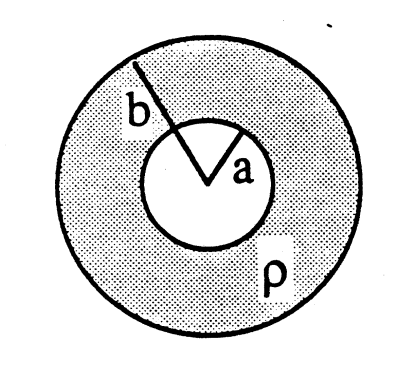
\includegraphics[scale=0.7]{01.png}
	\end{center}
\end{problem}
\begin{solution}
\end{solution}

\newpage
\begin{problem}[SUP27*]
	Consider the configuration of conductors shown in the figure below. All shaded areas are conductors and the total charges on each conductor are shown. Determine the distribution of the charges on all the relevant surfaces. Base your arguments on Gauss' law and show how you arrived at your answers.
	\begin{center}
		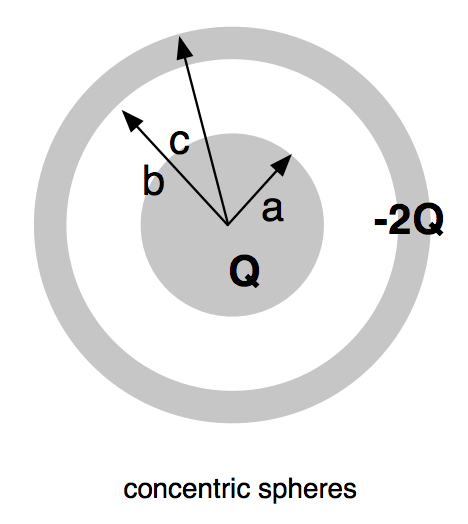
\includegraphics[scale=0.7]{02.png}
	\end{center}
\end{problem}
\begin{solution}
\end{solution}


\end{document}
